\documentclass[12pt]{article}
\usepackage[square,numbers]{natbib}     % package utilisé pour la partie de référence
\bibliographystyle{plainnat}
\usepackage[utf8x]{inputenc}
\usepackage[french]{babel}
\usepackage{caption}
\usepackage{subcaption}
\usepackage{url}
\usepackage{amsmath}
\usepackage{graphicx}
\graphicspath{{images/}}
\usepackage{parskip}
\usepackage{fancyhdr}
\usepackage{vmargin}
\usepackage[T1]{fontenc}

%Configuration pour les codes insérés
\usepackage{listings}
%\usepackage{color}
\lstset{frame=tb,
  language=Java,
  aboveskip=3mm,
  belowskip=3mm,
  showstringspaces=false,
  columns=flexible,
  basicstyle={\small\ttfamily},
  numbers=none,
  numberstyle=\tiny\color{gray},
  keywordstyle=\color{blue},
  commentstyle=\color{dkgreen},
  stringstyle=\color{black},
  breaklines=true,
  breakatwhitespace=true,
  tabsize=3
}


% utiliser pour faire annexe https://www.jujens.eu/posts/2013/Oct/20/latex-annexe/
% [titletoc permet d'afficher dans le table of contents]
\usepackage[titletoc]{appendix}

% make a clibable table of content
\usepackage[colorlinks=false]{hyperref}

%Includes "References" in the table of contents
\usepackage[nottoc]{tocbibind}

\usepackage{float} % utiliser cet package pour insérer les figures, permet de mettre juste après le texte

% Ce package est pour définir les couleurs de texte
\usepackage{xcolor}

%change paragraph indent
\setlength{\parindent}{2em}

\usepackage{vmargin}
%1 est la marge gauche
%2 est la marge en haut
%3 est la marge droite
%4 est la marge en bas
%5 fixe la hauteur de l’entête
%6 fixe la distance entre l’entête et le texte
%7 fixe la hauteur du pied de page
%8 fixe la distance entre le texte et le pied de page
\setmarginsrb{3 cm}{2.5 cm}{3 cm}{2.5 cm}{2 cm}{1.5 cm}{1 cm}{1.5 cm}

\title{\textbf{Rapport de projet de fin d'études\newline Automatisation de Test fonctionnel}}    % Title
\author{ZHANG Qilin}		% Author
\date{Septembre 2019}				% Date

\makeatletter
\let\thetitle\@title
\let\theauthor\@author
\let\thedate\@date
\makeatother

\pagestyle{fancy}
\fancyhf{}
\usepackage{lastpage}


\setcounter{tocdepth}{3} % Set the depth of table of contents
\setcounter{page}{3}
\begin{document}

%%%%%%%%%%%%%%%%%%%%%%%%%%%%%%%%%%%%%%%%%%%%%%%%%%%%%%%%%%%%%%%%%%%%%%%%%%%%%%%%%%%%%%%%%

\begin{titlepage}
	\centering
    \vspace*{0.5 cm}
    \begin{figure}
        \begin{subfigure}{0.3\textwidth}
        \flushleft
            
\includegraphics[width=\textwidth]{Logo_officiel_Sorbonne_University.png}
        \end{subfigure}
        \hspace{.4\textwidth}
        \begin{subfigure}{0.3\textwidth}
            
\includegraphics[width=\textwidth]{SAP_R_grad.jpg}
        \end{subfigure}
    \end{figure}
    \textsc{\LARGE Sorbonne Université}\\[2.0 cm]	% University Name
	\textsc{\Large Master 2 Science et Technologie du Logiciel\\2018 - 2019}\\[0.5 cm]		% Course Code
	%\textsc{\large Développement d'Application Réticulaire }\\[0.5 cm]	% Course Name
	\rule{\linewidth}{0.8 mm} \\[0.6 cm]
	{ \huge \bfseries \thetitle}\\
	\rule{\linewidth}{0.8 mm} \\[2.6 cm]

	\begin{minipage}{0.4\textwidth}
		\begin{flushleft} \large
			\emph{Etudiants:}\\
			\theauthor
			\end{flushleft}
			\end{minipage}~
			\begin{minipage}{0.4\textwidth}
			\begin{flushright} \large
			\emph{Tuteurs:} \\
			CHRISTIANSEN Camilla, COUDRAY Sébastien % Your Student Number
		\end{flushright}
	\end{minipage}\\[2.5 cm]
	 
	{\large \thedate}\\[2 cm]
 
	\vfill
	
\end{titlepage}
%%%%%%%%%%%%%%%%%%%%%%%%%%%%%%%%%%%%%%%%%%%%%%%%%%%%%%%%%%%%%%%%%%%%%%%%%%%%%%%%%%%%%%%%%
\null
\newpage
%%%%%%%%%%%%%%%%%%%%%%%%%%%%%%%%%%%%%%%%%%%%%%%%%%%%%%%%%%%%%%%%%
\pagenumbering{roman} % Start roman numbering

%% set thing show in right and left head and foot of page
\rhead{\rightmark}
\lhead{Sorbonne Université Master 2 STL\newline \theauthor}
\cfoot{\thepage}

%% set head and foot rule
\renewcommand{\headrulewidth}{2pt}
\renewcommand{\footrulewidth}{1pt}


\tableofcontents
\pagebreak

\listoffigures
\listoftables

\pagebreak

%%%%%%%%%%%%%%%%%%%%%%%%%%%%%%%%%%%%%%%%%%%%%%%%%%%%%%%%%%%%%%%%%%%%%%%%%%%%%%%%%%%%%%%
\pagenumbering{arabic} % Start roman numbering

\cfoot{Page \thepage \ sur\ \pageref{LastPage}}
\newpage
\section{Remerciements}
Je tiens tout d'abord à remercier toutes les personnes qui m'ont aidé au succès de mon alternance de cette année.

\par Je voudrais dans un premier temps remercier à l'ensemble de l'équipe \textit{Financier} de SAP France, pour son accueil et sa bienveillance tout au long de l'année. Je tiens à remercier particulièrement des personnes suivantes : 
\begin{itemize}
    \item Monsieur Sébastien Coudray et Madame Camilla Christiansen, mes tuteurs, avec qui que je travaille tout au long de l'année, pour leurs esprits professionnels, leurs patiences pour m'expliquer et m'aider pour mon travail.
    \item Monsieur David Dufour, 
    \item Thibault Lefaix
    \item Thierry Gosselin,
\end{itemize}

\par Mes remerciements ne sont pas envoyées que les personnes indiquées dans la liste précédentes, y contient aussi tous les collègues d'équipe, durant cette année de travail, ils m'ont aidé à bien "On-Boarding" à SAP France, m'ont aidé à déboguer mes programmes, m'ont pris le temps pour discuter mon sujet d'alternance. 

\par Je remercie également toute l'équipe pédagogique de Sorbonne Université et de CFA-INSTA, particulièrement monsieur Binh-Minh Bui-Xuan et monsieur Emmanuel Chailloux pour leurs conseils
tout au long de l’année, madame Emilie Auger pour son travail administrative de la promotion. Je remercie aussi la promotion M2 STL 2018 auprès de laquelle j’ai passé une année formidable

\par Enfin, je pense à mes proches, mes meilleurs amis, qui m'ont encouragé et soutenu pour ma vie et mes études en France tout au long de ces années.

%%%%%%%%%%%%%%%%%%%%%%%%%%%%%%%%%%%%%%%%%%%%%%%%%%%%%%%%%%%%%%%%%%%%%%%%%%%%%%%%%%%%%%%%%
\newpage
\section{Introduction}
\subsection{Cadre}
Ce rapport est écrit dans le cadre de ma formation en Master 2 Informatique à l'Université Sorbonne, dans ce cadre, j'effectue une année d'alternance chez SAP-France, intégré dans l'équipe 


\subsection{Organisation du rapport}
Ce rapport est divisé globalement en 6 parties, d'abord 

\newpage
%%%%%%%%%%%%%%%%%%%%%%%%%%%%%%%%%%%%%%%%%%%%%%%%%%%%%%%%%%%%%%%%%%%%%%%%%
\section{Présentation d'entreprise}

\subsection{Vue globale}
    \par SAP SE (\textit{\textbf{S}ysteme, \textbf{A}nwendungen und \textbf{P}rodukte in der Datenverarbeitung}, "\textbf{S}ystems, \textbf{A}pplications \& \textbf{P}roducts in Data Processing") est une entreprise qui conçoit et vend des logiciels, notamment des systèmes de gestion et de maintenance, principalement à destination des entreprises et des institutions dans le monde entier. SAP est une entreprise internationale et sont siège se trouve à Waldorf, Allemagne, SAP est le premier éditeur de logiciels en Europe et le quatrième dans le monde.
    
    \par SAP a XXXX d'employées, XXX (\underline{Présentation sur la bourse, l'influence mondiale, nombre d'employés, etc.})
\subsection{Histoire}
Sources : \citet{SAP-History}
    \subsubsection{Années 1972 - 1980: Les jeunes années}
    En 1972, 5 anciens employés d'IBM - Dietmar Hopp, Hans-Werner Hector, Hasso Plattner, Klaus E. Tschira, et Claus Wellenreuther - fondaient Systems Applications and Products in Data Processing (Systèmes, Applications et Progiciels), à Mannheim, en Allemagne. S'appuyant sur le rêve de l'informatique «temps réel»: un logiciel qui traite les données lorsque les clients en ont besoin plutôt que de passer la nuit à la volée. SAP a délivré la release SAP R/1 en 1973.

    \subsubsection{Années 1981 - 1990 : Le SAP R/2}
    Le temps réel touche davantage l’activité: les processus d’application logicielle mainframe packagés SAP R/2 intègrent l’ensemble des fonctions commerciales d’une entreprise.

    \subsubsection{Années 1991 - 2000 : Le SAP R/3}
    Temps réel sur le bureau: une version client-serveur du logiciel d'application standard permet aux entreprises de fonctionner plus efficacement dans le monde entier.
    \subsubsection{Années 2001 - 2010 : Des données en temps réel}
    Déplacements vers le Web en temps réel et au-delà: l'informatique en nuage, mobile et en mémoire ouvrent de nouveaux horizons pour l'accès aux données en temps réel, où que vous soyez et quand vous en avez besoin.
    
    \subsubsection{Année 2011 - Présent : Résultats d'enregistrement des supports de prise en charge en mémoire, en nuage et en réseau d'entreprise}
    La croissance continue de l'entreprise est tirée par la plate-forme en mémoire SAP HANA qui permet aux analyses de données ultra-rapides de devenir une réalité. Des acquisitions stratégiques associées à une innovation continue font de SAP un leader des réseaux d’informatique en nuage et du commerce électronique. Avec le lancement de SAP S / 4HANA et de SAP C / 4HANA, SAP dévoile la nouvelle génération de logiciels d'entreprise destinés à aider les clients à devenir des entreprises intelligentes.

\subsection{Commerce de SAP} 
\subsubsection{Activités et marchés}
\cite{SAP-entreprise_wikipedia}SAP opère dans trois zones géographiques : Europe/Moyen-Orient/Afrique (\textbf{EMEA}), \textbf{Amériques} (le siège de SAP America, qui regroupe Amérique du Nord et Amérique latine, se trouve à Newtown Square, en Pennsylvanie), et Asie/Pacifique/Japon (\textbf{APJ}, qui regroupe Japon, Australie, Inde et plusieurs autres pays d’Asie). SAP dispose également d’un réseau de 115 filiales, et de cabinets de Recherche \& Développement.

SAP se concentre sur six secteurs : procédés industriels de fabrication, d’assemblage, de distribution et de services aux consommateurs, services financiers et publics21[source insuffisante]. La société propose plus de 25 produits aux grandes entreprises et plus de 550 pour les petites et moyennes entreprises.

Les différents départements opérationnels de SAP sont divisés en trois catégories : Recherche \& Développement, activités de terrain et assistance aux consommateurs. SAP Labs conçoit et développe les produits, tandis que des bureaux installés dans chaque pays partenaire se chargent des opérations de terrain comme la vente, le marketing et le conseil. La stratégie et la gestion globale sont décidées et menées au siège de SAP AG, en Allemagne, tout comme le travail d’ingénierie lié à la fabrication des produits.

\subsubsection{Produits \& Services}
\subsection{SAP Aujourd'hui et Demain}
La partie plus important que les autres, moins d'histoire.

\subsection{SAP France}
    \subsubsection{SAP Labs in Paris}

    \subsubsection{Equipe DEV Paris}
    
        \paragraph{Organisation du groupe}
        \begin{figure}[H]
            \centering
            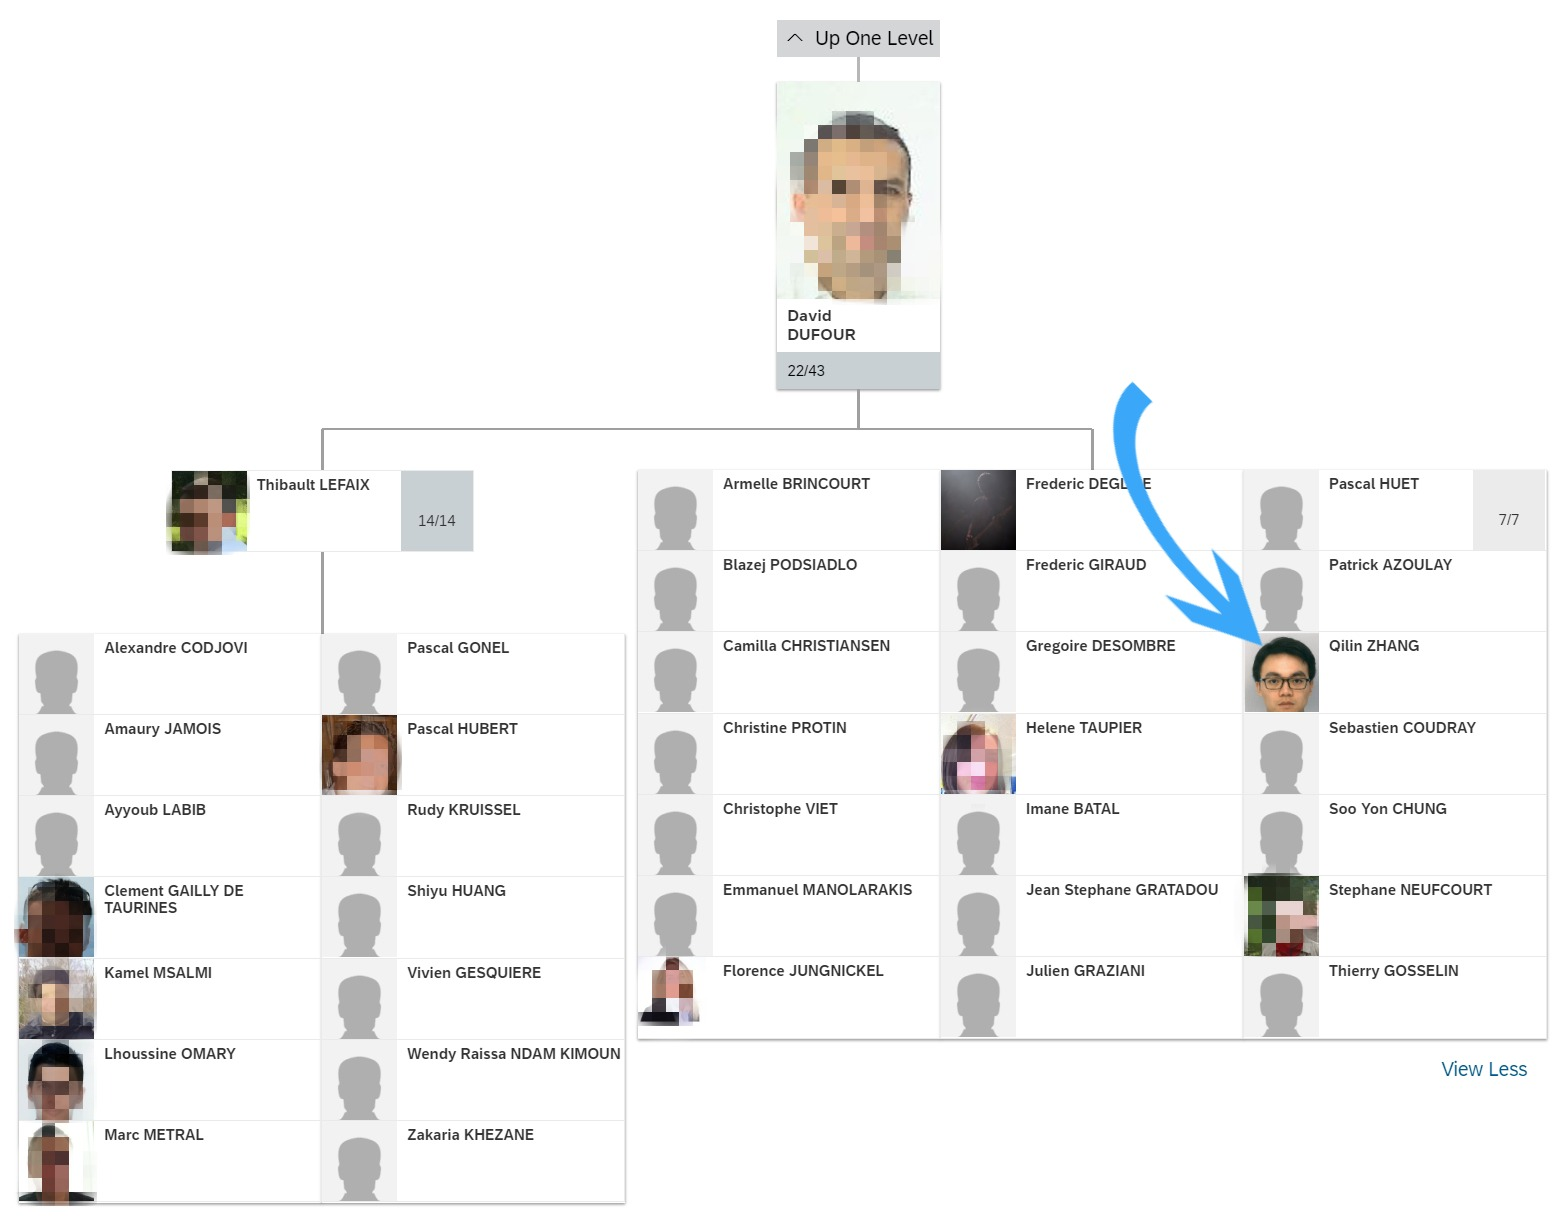
\includegraphics[width=\textwidth]{organisation_groupe.jpg}
            \caption{Organisation du groupe}
            \label{fig:my_label}
        \end{figure}
        
        \paragraph{Mon rôle et ma mission}
        \newpage

\section{Compréhension de la problématique}

\subsection{SAP Financial Consolidation}
    \subsubsection{Consolidation financière}
    
    \subsubsection{Architecture}
    Contient Client Lourd, Client Web Legacy, Client HTML5
    
    \subsubsection{Méthodologie du travail - Agile}\par
    L'équipe travaille avec la méthode d'Agile, qui est s'adapte très bien aux besoins du projet. Nous avons un tableau de mission collé sur mur qui indique l'avancement de chaque mission comme suivant : 
    \begin{figure}[H]
        \centering
        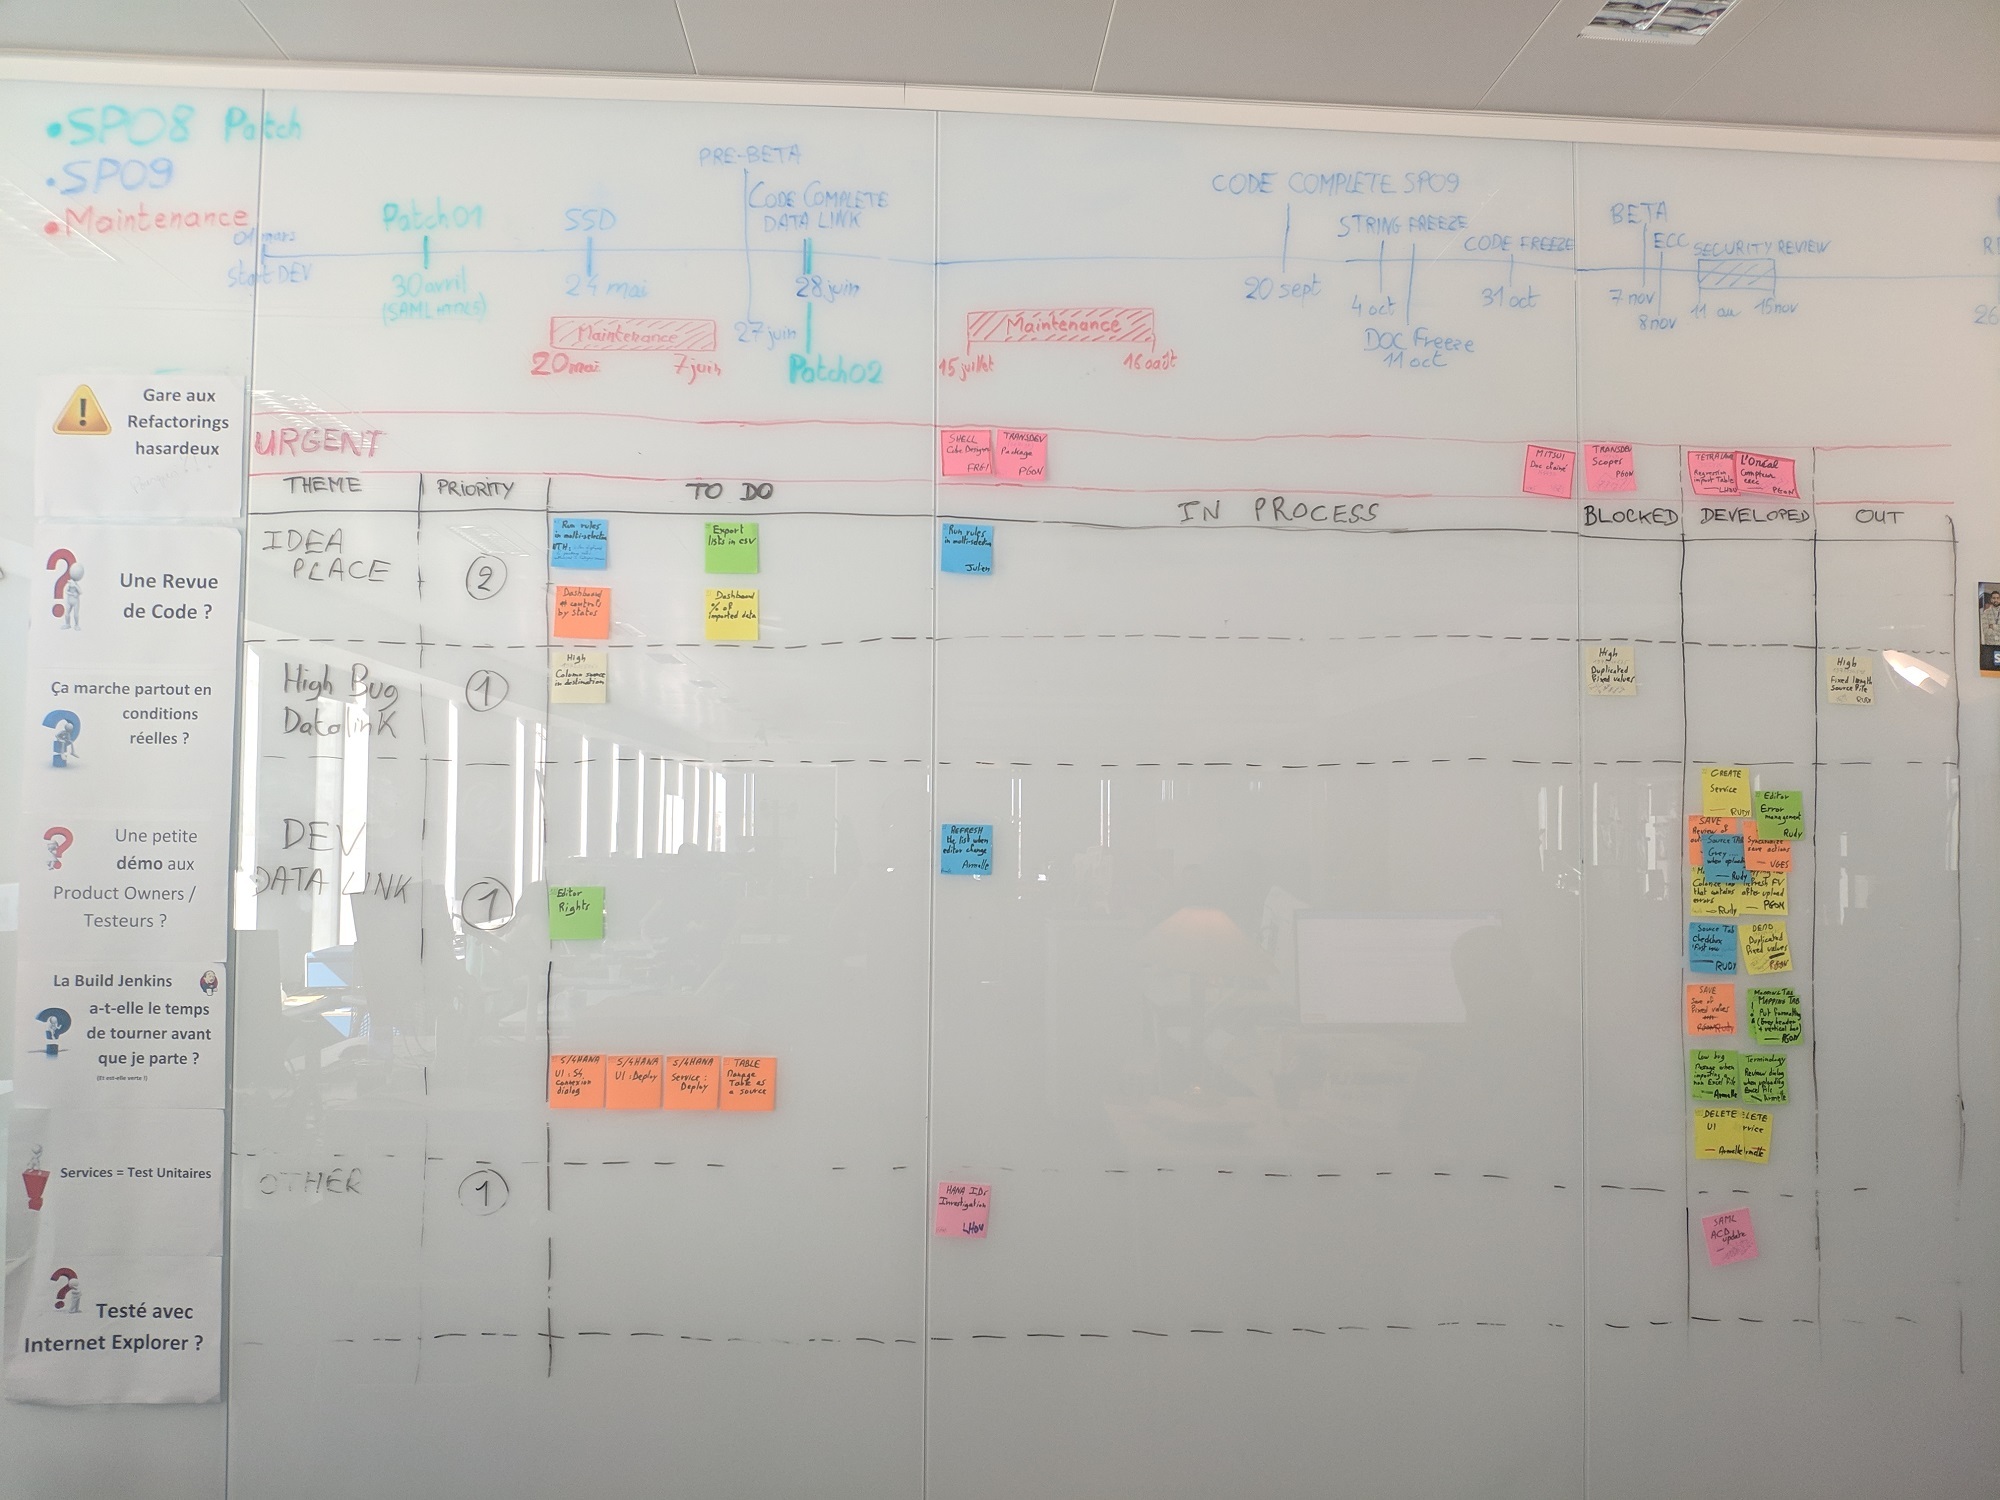
\includegraphics[width=\textwidth]{scrum_tachTable.jpg}
        \caption{Scrum - Table des tâches}
        \label{fig:scrum_figure}
    \end{figure}
    \par Chaque jour pendant 13h40 et 14h20, notre Scrum Master Thierry XXXX organise une "Stand-up" avec \textit{Skype for Business} réunion que tous les membres d'équipe participent et restent debout au cours de laquelle chacun répond principalement à 3 questions : « Qu'est ce que j'ai terminé depuis la dernière réunion ? Qu'est ce que j'aurai terminé d'ici la prochaine réunion ? Quels obstacles me retardent ? »
    
    \subsubsection{Build et Livraison, Maintenance et Update}
    Le produit FC n'est pas une \textit{Continnous  Integration} et \textit{Continuous Delivry}
    
    %\subsubsection{Test Automatisé}
    
    %\subsubsection{Maintenance}

    \subsubsection{Outils utilisés}
        \paragraph{Gestion du code - PERFORCE}
            \par Pour la gestion de version du code, nous utilisons Perforce.
            \begin{figure}[H]
                \flushleft
                
\includegraphics[width=.3\textwidth]{Perforce_Logo.jpg}
                \label{fig:Perforce_Logo}
            \end{figure}
            \par Perforce est un outil de gestion de configuration utilisé dans le processus de développement logiciel. Nous utilisons un des ces outils Helix Visual Client (P4V), Helix Visual Client (P4V) est une application de bureau qui permet d’accéder aux fichiers versionnés dans Helix Core via un interface graphique. Il comprend des outils permettant de fusionner et de visualiser l'évolution du code.
            \par Avec P4V, il est facile de personnaliser notre espace de travail afin de ne voir que les fichiers dont nous avons besoin. Nous pouvons travailler hors ligne et à distance. Et lorsque nous avons terminé, transférez facilement les modifications locales sur un serveur distant. 
            \newline 
            Nous pouvons : \newline
            \begin{itemize}
                \item Voir les changements de time-lapse et de révision. 
                \item Obtenez un aperçu des métadonnées du projet.
                \item Demander des révisions de code sur les modifications en attente.
            \end{itemize} 
            \par Dans notre équipe, chaque remonte du code est revue par l'autre développeur, pour moi, c'est mon encadrant technique Sébastien Coudray relit mes codes. 
        \paragraph{Edition du code - Eclipse}
        Avec la raison d'utilisation plugin Silk4J, nous avons choisissons d'utiliser Eclipse comme éditeur du code.
            \begin{figure}[H]
                \flushleft
                
\includegraphics[width=.3\textwidth]{Eclipse_logo.png}
                \label{fig:eclipse_logo}
            \end{figure}
        \paragraph{Outil de Testauto : SilkTest - Silk4J}
        \par Silk Test est un outil de test de fonction automatisé et de régression des applications d'entreprise.
    
        \paragraph{Intégration continue - Jenkins}
        \paragraph{Environnement de Testauto - Machines virtuelles}
        \paragraph{Partage de fichiers et e'informations - One Drive }
        \paragraph{Communication interne - Skype for Business + Outlook}

%%%%%%%%%%%%%%%%%%%%%%%%%%%%%%%%%%%%%%%%%%%%%%%%%%%%%%%%%%%%%%%%%%%%%%
\newpage

    \subsubsection{Langages et Technologies utilisées}
    \par Silk est déjà utilisé par une autre équipe, c'est la raison de choisir Silk, fin 2013.
    
    \par Pourquoi Java ? Préférence des développeurs, et Java est supporté par SilkTest.
    
    \par Faire un tableau de comparaison d'aujourd'hui et l'avenir, de Silk et Selenuim, etc.

%%%%%%%%%%%%%%%%%%%%%%%%%%%%%%%%%%%%%%%%%%%%%%%%%%%%%%%%%

\subsection{Client HTML5 : Test Manuel VS Test Automatisation}
Architecture de Test-Auto, schéma, Jenkins + Vm + BD + Code
\subsubsection{Procédure de test automatié sur les machines virtuelles}

\subsection{Test d'impression}
    \subsubsection{Analyse du problème}
    La raison pourquoi on choisit test-auto pour l'impression

\newpage
%%%%%%%%%%%%%%%%%%%%%%%%%%%%%%%%%%%%%%%%%%%%%%%%%%%%%%%%%%%%%%%%%%%%%%%%%
\section{Travail réalisé}
\subsection{Schéma global}

    \subsection{Etat de l'art}
    Etat du travail quand je suis arrivé
    \subsubsection{Silk4J + Codes en Java + JUnit}
    
    \subsubsection{Réalisation des scénarios des Tests}

\subsection{Développements}
    \subsubsection{Réalisation des scénarios de test avec Junit}
    
    \subsubsection{Codes de comparaison des PDF}
    Les codes récupés d'une autre équipe
    \subsubsection{Télécharger et décompresser un zip}
    
    \subsubsection{Comparaison les pdf dans deux répertoire avec Lambda Expression}

\newpage
%%%%%%%%%%%%%%%%%%%%%%%%%%%%%%%%%%%%%%%%%%%%%%%%%%%%%%%%%%%%%%%%%%
\section{Conclusion}

\newpage

%%%%%%%%%%%%%%%%%%%%%%%%%%%%%%%%%%%%%%%%%%%%%%%%%
\bibliography{biblist}

\newpage
\begin{appendix}

\section{Multi-Thread pour la comparaison des pdf}

\section{Lambda Expression pour comparaison entre deux répertoires}
\end{appendix}
\newpage

%\begin{center}
%    \includegraphics[width=\textwidth]{maquette_mainPage.png}
%\end{center}

\end{document}